\section{Apresentação}

Para apresentar os resultados, serão abordadas tabelas contendo testes com todas as combinações de imagens, uma imagem com os resultados finais das tabelas, além de uma imagem com todos os passos da aplicação.

A Tabela \ref{tab:final_input_output_2d} apresenta os resultados comparativos entre a imagem de entrada e o mapa 2D. Esta comparação é realizada utilizando a técnica de classificação de conjuntos, conforme definido por \cite{kirillov2019panoptic}. A análise foca na avaliação das métricas, conforme o número de pontos no diagrama de Voronoi, incluindo União sobre Interseção (IoU), Acurácia (Acc), F1 Score (F1), Coeficiente de Correlação de Matthews (MCC), Taxa de Descoberta Falsa (FDR), Taxa de Falso Negativo (FNR) e o tempo de execução do código \cite{Chicco2020, confusion_matrix_calculator, iou_metric_link}.

Esta tabela é crucial, pois ela evidencia, com base em dados concretos, a semelhança do mapa 2D com o contorno do mapa de entrada. Além disso, corrobora a hipótese de que um maior número de pontos no mapa leva a melhores resultados nas métricas de IoU, Acc, F1 e MCC (onde valores mais altos indicam melhor desempenho), e simultaneamente, a uma redução nos índices de FDR e FNR (onde valores menores são preferíveis, visto que representam menor erro). Observa-se, ainda, que um aumento no número de pontos implica em um maior tempo de processamento na geração procedural do mapa.

\begin{table}[h]
	\centering
	\caption{Resultados dos testes entre imagem de entrada e mapa 2d}
	\label{tab:final_input_output_2d}
	\begin{tabular}{|c|c|c|c|c|c|c|c|}
		\hline
						Pontos & IoU & Acc & F1 & MCC & FDR & FNR & Duração \\
		\hline
		50 & 0.71361 & 0.86085 & 0.8323 & 0.74079 & 0.2762 & 0.01923 & 5.33293\\
100 & 0.80033 & 0.9151 & 0.88857 & 0.82809 & 0.17938 & 0.0292 & 10.0857\\
150 & 0.83825 & 0.93506 & 0.91168 & 0.86398 & 0.13792 & 0.03125 & 15.32477\\
200 & 0.85695 & 0.94434 & 0.92268 & 0.88059 & 0.10822 & 0.04269 & 20.22667\\
250 & 0.868 & 0.94946 & 0.92908 & 0.89029 & 0.09454 & 0.04525 & 27.26459\\
300 & 0.87405 & 0.95241 & 0.93263 & 0.89612 & 0.08326 & 0.04984 & 33.46705\\
		\hline
	\end{tabular}
\end{table}


Os resultados obtidos na \cref{tab:final_input_output_3d} derivam da comparação entre a imagem de entrada e o mapa de altura, utilizando a técnica de classificação de conjuntos conforme definida por \cite{kirillov2019panoptic}. Essa comparação foi realizada para mensurar diversos aspectos, incluindo as métricas associadas ao número de pontos no diagrama de Voronoi. As métricas abrangem União sobre Interseção (IoU), Acurácia (Acc), F1 Score (F1), Coeficiente de Correlação de Matthews (MCC), Taxa de Descoberta Falsa (FDR), Taxa de Falso Negativo (FNR) e a duração da execução do código \cite{Chicco2020, confusion_matrix_calculator, iou_metric_link}.

A relevância dessa tabela reside na capacidade de demonstrar, por meio de dados concretos, a proximidade entre o mapa de altura e o contorno do mapa de entrada. Além disso, ela valida a hipótese de que o aumento no número de pontos resulta em melhores desempenhos nas métricas de IoU, Acc, F1 e MCC, indicando uma maior semelhança entre os mapas. Simultaneamente, observa-se uma diminuição nas métricas de FDR e FNR, evidenciando uma redução nos erros. Vale notar que a quantidade de pontos também impacta diretamente na duração da geração procedural do mapa, sendo um fator relevante a ser considerado.


\begin{table}[h]
	\centering
	\caption{Resultados dos testes entre imagem de entrada e mapa de altura}
	\label{tab:final_input_output_3d}
	\begin{tabular}{|c|c|c|c|c|c|c|c|}
		\hline
						Pontos & IoU & Acc & F1 & MCC & FDR & FNR & Duração \\
		\hline
		50 & 0.67955 & 0.83753 & 0.80827 & 0.70471 & 0.31036 & 0.02058 & 5.29547\\
100 & 0.74929 & 0.88637 & 0.85581 & 0.77953 & 0.23518 & 0.02501 & 9.822\\
150 & 0.79092 & 0.91133 & 0.88236 & 0.82054 & 0.18669 & 0.0319 & 15.43131\\
200 & 0.80368 & 0.91818 & 0.89056 & 0.83234 & 0.17252 & 0.03302 & 21.06372\\
250 & 0.82316 & 0.92831 & 0.90248 & 0.85016 & 0.14821 & 0.03784 & 25.92615\\
300 & 0.82598 & 0.93022 & 0.90415 & 0.85286 & 0.14182 & 0.04223 & 32.75651\\
		\hline
	\end{tabular}
\end{table}

A tabela referenciada como \cref{tab:final_output_2d_output_3d} apresenta os resultados comparativos entre o mapa de altura e sua representação em mapa 2D. Esta comparação é realizada através do método de classificação de conjuntos proposto por \cite{kirillov2019panoptic}, avaliando os resultados com base em várias métricas conforme a quantidade de pontos no diagrama de Voronoi. As métricas avaliadas incluem União sobre Interseção (IoU), Acurácia (Acc), F1 Score (F1), Coeficiente de Correlação de Matthews (MCC), Taxa de Descoberta Falsa (FDR), Taxa de Falso Negativo (FNR) e o tempo de execução do código \cite{Chicco2020, confusion_matrix_calculator, iou_metric_link}. Esta tabela é crucial para demonstrar que o mapa de altura, que se transformará no mapa 3D, assemelha-se ao mapa 2D. Essa similaridade é fundamental no protótipo do Unity para a localização do personagem, combinando o mapa 2D como minimapa e o mapa 3D com dimensão e profundidade. Observa-se também que um aumento no número de pontos resulta em maior tempo de geração procedural do mapa.


\begin{table}[h]
	\centering
	\caption{Resultados dos testes entre mapa 2d e mapa de altura}
	\label{tab:final_output_2d_output_3d}
	\begin{tabular}{|c|c|c|c|c|c|c|c|}
		\hline
						Pontos & IoU & Acc & F1 & MCC & FDR & FNR & Duração \\
		\hline
		50 & 0.91515 & 0.9589 & 0.95559 & 0.91721 & 0.06528 & 0.0222 & 5.0949\\
100 & 0.90352 & 0.95708 & 0.94924 & 0.91312 & 0.08082 & 0.01838 & 10.08713\\
150 & 0.90342 & 0.9592 & 0.94915 & 0.91636 & 0.08265 & 0.01631 & 14.82656\\
200 & 0.90421 & 0.96087 & 0.94955 & 0.91901 & 0.08312 & 0.01487 & 20.51247\\
250 & 0.90505 & 0.96207 & 0.95004 & 0.92088 & 0.08284 & 0.0142 & 26.63407\\
300 & 0.90357 & 0.96252 & 0.94921 & 0.92112 & 0.08565 & 0.01276 & 33.59293\\
		\hline
	\end{tabular}
\end{table}

A \cref{fig:result_final} contém a ilustração da classificação dos conjuntos de cada combinação. Assim, a imagem (a) ilustra a última execução da combinação entre a imagem de entrada e o mapa 2D, conforme os resultados da \cref{tab:final_input_output_2d}. A imagem (b) exibe a última execução da combinação entre a imagem de entrada e o mapa de altura, conforme os resultados da \cref{tab:final_input_output_3d}. Já a imagem (c) apresenta a última execução da combinação entre o mapa de altura e o mapa 2D, conforme os resultados da \cref{tab:final_output_2d_output_3d}.

\begin{figure}[!ht]
	\centering
    \caption{Resultados da última execução de cada combinação de imagens.}
	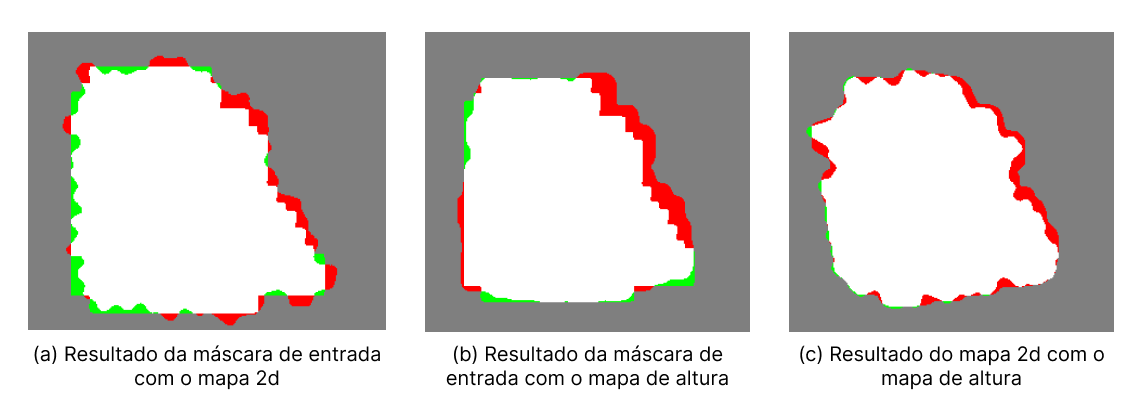
\includegraphics[width=\textwidth]{figures/comb_results_final.png}
    \legend{Fonte: \space Autoria própria}
	\label{fig:result_final}
\end{figure}

A \cref{fig:combs_result} apresenta todos os passos da execução do programa gerado em Python. A imagem (a) mostra uma captura de tela da interface gráfica com PyQt5. A imagem (b) exibe uma captura de tela do processo de abertura de uma imagem para segmentação. Na imagem (c), é apresentada uma captura de tela da execução do modelo EfficientPS na imagem selecionada. A imagem (d) mostra uma captura de tela da saída da segmentação panóptica pelo modelo EfficientPS. Na imagem (e), temos o carregamento pós-seleção do usuário, que, no caso, selecionou um carro com o método de preenchimento por inundação. A imagem (f) exibe o resultado do mapa 2D com o contorno selecionado anteriormente. Na imagem (g), é apresentada uma captura de tela da automação usando Unity para atualizar um terreno com o mapa de altura resultante da geração procedural. Por fim, a imagem (h) mostra uma captura de tela do Unity rodando a aplicação e abrindo o minimapa (usando o mapa 2D) para oferecer uma noção de localização no mapa 3D, usando um ponto para marcar a localização atual do personagem no minimapa (mapa 2d).


\begin{figure}[!ht]
	\centering
    \caption{Passos do programa final.}
	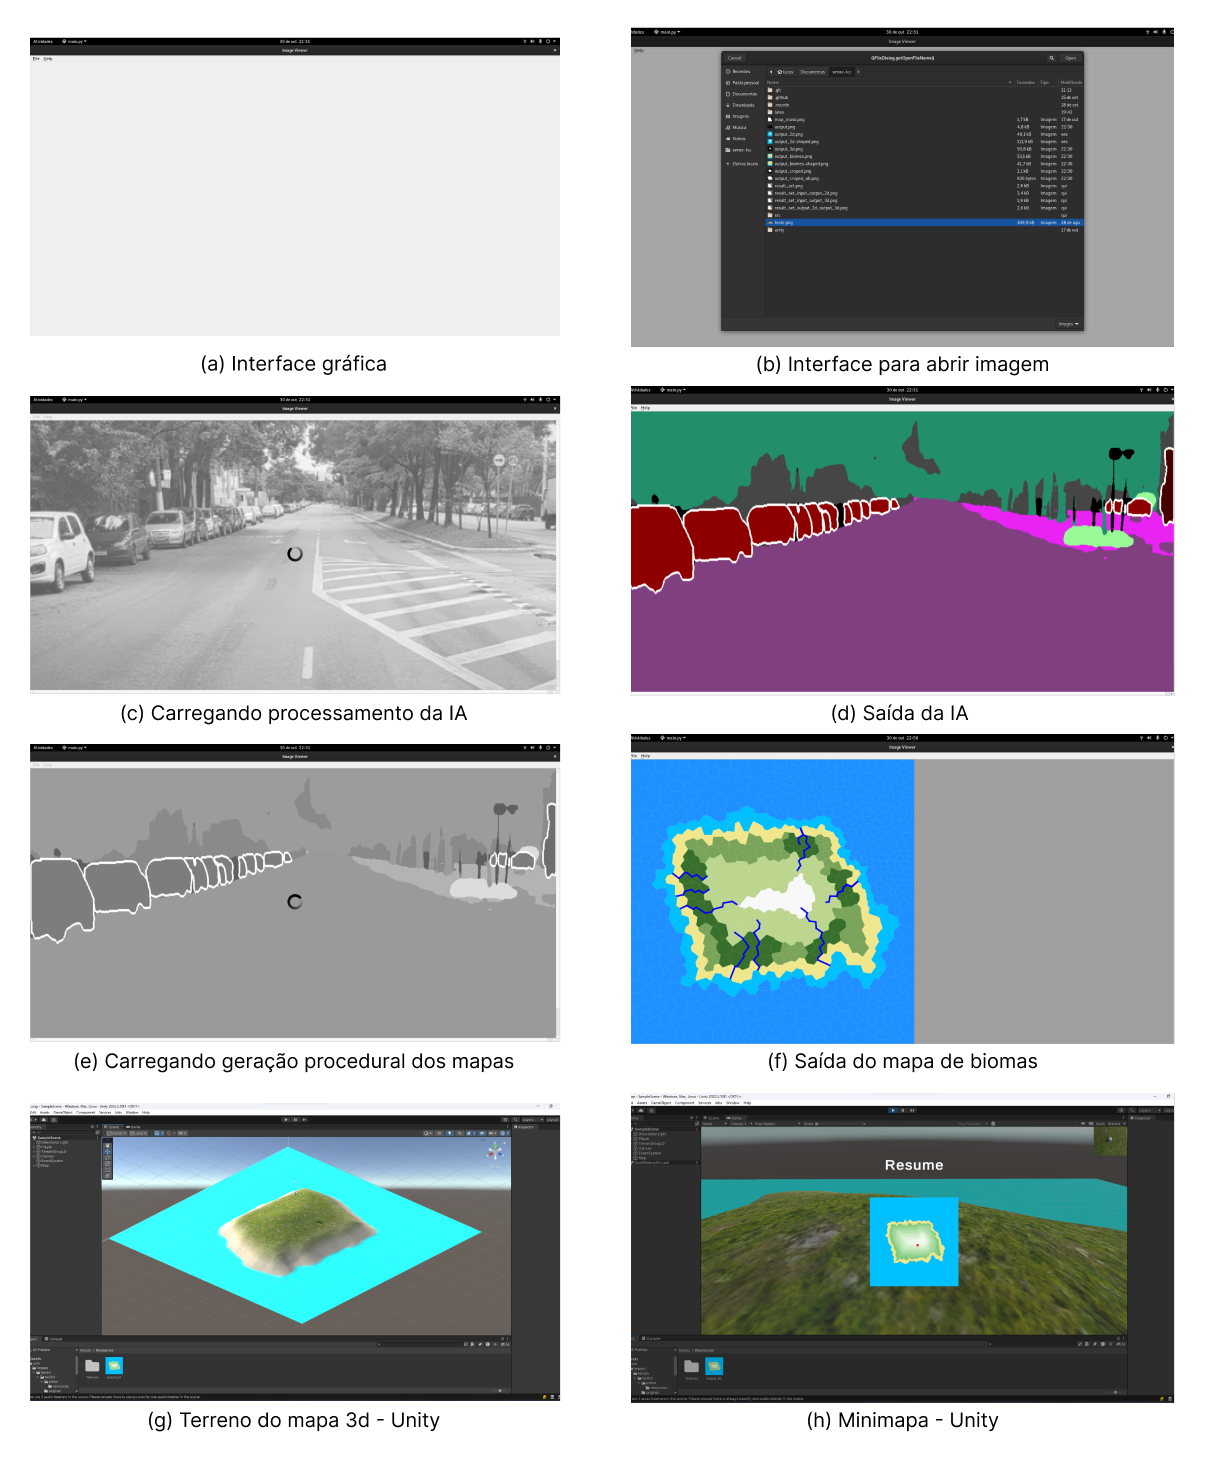
\includegraphics[width=\textwidth]{figures/result_final.png}
    \legend{Fonte: \space Autoria própria}
	\label{fig:combs_result}
\end{figure}